\chapter{A Medical Case Study}\label{c:medical-study}

In this thesis we primary focus to analyze medical data by using some of the aforementioned techniques from section \ref{c:preliminaries}.
More specifically we have developed a complete platform built around secure medical data analytics that could be beneficial to patients, doctors and researchers.

The platform can provide insights about some medical datasets that are imported into the platform to anyone who wants to query them, without compromising individual patient's privacy.
These analytics which include data aggregation / statistics and classification are implemented through privacy preserving algorithms under the secure multi-party computation scenario.

The platform provides end to end work flow starting from the query selection from a user.
Following is the secure data importing, the performing of privacy preserving data analytics algorithms upon those data and finally the visualization of the results to the end user through a friendly user interface (UI).

\section{A Doctor's view}
We consider the use case of a doctor working in a hospital that wants to examine the data stored in that hospital's datasets.
He/She could possibly want to evaluate a treatment's outcome.
To achieve this, the doctor should have monitored some particular datasets in order to have an overall view of the patients' condition over time.
This could allow a comparison between previously treated patients and enable data-driven cues for the treatment.
For example, a drug's effect could be evaluated that way.

The doctor could also compare aggregate results from datasets between different hospitals.
That way he/she could get an insight of how each patients' condition varies between different hospitals, which could indicate the different effect that different treatments have on patients and identify patterns
and differences in these treatments.

Continuous monitoring of patient data is useful for any hospital.
Provided with usable and informative tools a doctor could potentially make better diagnoses and take the appropriate action for each case.


\section{An Individual's view}
An individual could also benefit from the insights provided by our platform.
We consider the case in which an individual with a certain condition queries the available datasets looking for the same condition.
The individual could locate the hospitals in which patients with the same condition are treated.
Also, he/she could identify which hospitals in his area have the best outcome for patients with conditions similar to his/hers.


Another way an individual could be benefited from the privacy preserving medical data analytics is the use of a classification mechanism using a model trained over patient data.
This way one could classify himself to a condition / disease or another chosen attribute for that matter, based on his own data.


\section{A Researcher's view}
We examine the case where an academic or industry researcher queries the datasets to see if they suit their research needs.
They could discover if the datasets are providing enough utility / information and decide which ones to use for performing analysis on.

For example, studying aggregate statistical information of the datasets, one could find possible correlations of particular attributes or find patterns of treatments and conditions.

A researcher could also study the relation between certain conditions and different hospitals, which is something that could provide valuable information.



\section{Our architecture \fixme{give a fancy name for the whole scheme.}}\label{s:architecture}
Our architecture consists of the \textit{SMPC cluster}, a proxy server, dubbed \textit{coordinator}, as well as \texttt{N} more servers that are hosted in the hospitals' premises and act as \textit{data providers}.

\textbf{SMPC cluster}: The \textit{SMPC cluster} consists of three servers -- three computing nodes -- participating in the SMPC protocol.
In our case, these nodes do not provide the data for the computation.
The only data the computing nodes hold and process, are cryptographic shares of the original data obtained through the secret-sharing mechanism.

\textbf{Data providers}: The \textit{data providers} are hospitals that provide medical datasets upon which the privacy preserving algorithms will execute.
When the medical data are transferred from the hospitals to the computing nodes, they get secret\hyp shared.


\textbf{Coordinator}: The \textit{coordinator} handles all private computation requests.
The server listens for requests for private query execution, and when such a request arises, the coordinator communicates with the data providers (all \texttt{N} hospitals) requesting them to securely import their data to the computing cluster.
The data are then secret\hyp shared to the three nodes, with each node acquiring one share of the original value.
Then the privacy preserving computation takes place in the SMPC cluster, and the results get visualized and served back to the requesting user through the \textit{coordinator} server.


\subsection{End-to-End Execution Flow}\label{ss:end-to-end-execution-flow}

An overview of an end\hyp to\hyp end query execution can be found below.

\begin{description}[labelwidth=4em, leftmargin=\dimexpr\labelwidth+\labelsep\relax]
    \item [Step 1:] A user makes a privacy\hyp preserving analytics request to the \textit{coordinator}.
    \item [Step 2:] The \textit{coordinator} server is responsible for orchestrating all the involved parties: it communicates with the data\hyp providers requesting secure data\hyp import to the SMPC cluster.
    \item [Step 3:] The data\hyp providers extract the requested data from their datasets and securely import them to the SMPC cluster applying secret\hyp sharing.
    \item [Step 4:] The SMPC cluster computes the privacy preserving analytics on the requested data and returns the results to the \textit{coordinator}.
    \item [Step 5:] Finally, the results are returned to the user through the \textit{coordinator}.
\end{description}

In the subsequent section we delve into the above end\hyp to\hyp end execution overview in more detail.


\subsubsection{Query Initiation}\label{sss:query-initiation}
First, a user sends a request to the \textit{coordinator} asking for a private computation.
This user can be an analyst / researcher, a doctor, or a patient.
This request can specify any one of the supported privacy preserving computations.

Users get informed about the available privacy preserving analytics algorithms through the \fixme{TheFancyName} User Interface (UI).
The UI is responsible to inform the user about the supported computations, as well as the available datasets on which these computations can be executed.
These datasets are populated from the hospitals that participate in the platform.

The user's request includes the desired private computation to be executed, the selected attributes that are involved in this computation, as well as the selected datasets.

\subsubsection{Data Import}\label{sss:data-import}

After the coordinator server collects the user's private computation query, a data importing procedure takes place.

The server will send an importing request to the hospitals that are specified in the user's query.
The importing request will include the attributes indicated by the user that are participating in with the private computation.

Upon receiving such an importing request, each hospital involved in this private computation will import a part of its dataset, that is associated with the participating attributes, into the SMPC cluster.
The data to be imported will be secret\hyp shared between the nodes participating in the SMPC protocol, using an additive secret\hyp sharing protocol.

The data importing is a procedure of high importance, since the patients' data are transferred outside the hospitals to third party servers.
It is easily misinterpreted that since the data are leaving the hospitals' premises, their privacy is being compromised.
However, it has been elucidated in section \ref{s:secret-sharing} that secret sharing is a form of encryption, thus no information leakage is possible while data being in use in the SMPC cluster.
For transferring each share from the data providers to the corresponding SMPC computing nodes standard techniques -- such as symmetric encryption -- are used to protect data in transit.
Data are also safe while at rest in the SMPC cluster as each node only stores a cryptographic share of a piece of data, so no information about the original data can be inferred.

\subsubsection{Computation Execution}\label{sss:computation-execution}

The next step after the data import is the actual private computation execution.
The nodes participating in the SMPC protocol, execute the privacy preserving version of the analytics algorithm that the requesting user has selected.

The algorithm is executed on encrypted (secret\hyp shared) data, thus the computing nodes have no access to the original data that still reside on the hospitals.
The execution is oblivious as far as the data is concerned.
Any data that gets published is explicitly defined in the privacy preserving algorithms and usually \footnote{Some data (e.g. those that will be included in the output) can be published before the algorithm terminates, without violating the prescribed privacy guarantees.} is only the computation output.

\subsubsection{Result Publishing}\label{sss:result-publishing}

The last step of the secure query execution is the publishing of the computation results.
These are obtained through computation over private data.
The results are now considered public data and can be freely shared with the user that requested the computation or be used in other future computations.
One thing to note is that every published result of such a computation should be treated as public data and should not be confused with the confidential input data.
With that in mind, whoever initiates a private computation should have a clear view of what data remain private and what gets published.


The detailed procedure described above is depicted in figure \ref{f:overview}.

\begin{figure}[t]
  \centering
  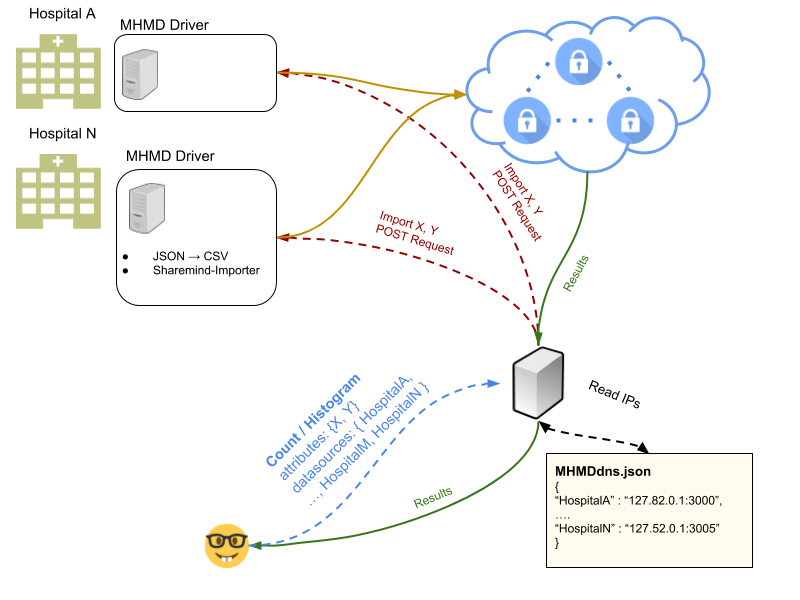
\includegraphics[width=\linewidth]{figures/overview.png}
  % \vspace{-0.2in}
  \caption{An overview of the architecture of our study \fixme{update to latest version: (not yet..)}}\label{f:overview}
\end{figure}



\subsection{SMPC Threat Model}\label{s:smpc-threat-model}
The main security goal of every SMPC engine is to protect the values provided by the input parties from all other parties.
The data of the input parties will be stored and processed encrypted by the computing parties.
The SMPC cluster needs to ensure that no party can learn anything from the information available to them.

Moreover, the final results must not reveal anything except for the actual results of the secure computation performed by the computing parties.
Note, that depending on the algorithm and provided data, the output may leak the input of one or more input parties.
For instance, without loss of generality let us suppose a SMPC setting with two parties.
A malicious adversary can always alter his/her input and define it to be an empty database (or a database with null values).
This fact can be very damaging since the final output is the result of the algorithm on the other party’s database alone.

In this work we assume that the adversary is \emph{semi\hyp honest} -- or similarly, \emph{rational, honest\hyp but\hyp curious}.
That is, the adversary correctly follows the protocol specification, but has incentives to eavesdrop sensitive user data.
He/She could also attempt to learn additional information by analyzing any data received during the execution, either unencrypted or encrypted.
In our developed algorithms, we explicitly define which variables are sensitive and should remain encrypted throughout the whole execution to preserve data privacy.


\subsubsection{Computing Parties Collusion}\label{s:computing-parties-collusion}
In the active adversary scenario, where the adversary controls some of the computing nodes, the only requirement is not to control all of them simultaneously.
Since the actual data are transferred from the data-providers (hospitals) to the computing nodes through secret\hyp sharing, it is impossible for any of the three nodes to decrypt them, and in general to infer any information, as each computing node possesses only a share of the data.
However, meaningful computations can be applied due to the homomorphic properties that the shares have (section \ref{ss:secret-sharing-homomorphism}).

As we examined in section \ref{s:smpc}, the computing nodes of the SMPC cluster do not need to be trusted nodes.
The only requirement of these nodes is not to collude.
This should not be confused with trusted servers.
A reasonable way to prevent collusion, is to deploy the computing nodes in premises of organizations having conflicting interests.

Finally, the only information that gets published is the output of the privacy preserving computation.
This is returned to the user who initiated the query via the \textit{coordinator} server.



\subsection{Data Importing On-the-Fly}\label{s:importing-otf}
Everyday, thousands of people visit their doctors, updating their medical records with new diagnoses.
One may wonder, \textit{since the medical data of each hospital are constantly changing, how often should the datasets in the SMPC cluster be updated?}

In our architecture, we have developed a mechanism for data importing \textit{on-the-fly}, as figure \ref{f:overview} portrays.
More specifically, when a query is requested for private computation, the coordinator interacts with the hospitals' servers, initiating the data import procedure.
Since the individual making the query also selects some specific attributes for data aggregation and/or classification, the importing of the data only happens for the selected attributes.

This importing on-the-fly is beneficial for many reasons.
First and foremost, all private computations are evaluated over the most recent data, and not in a former version of them.
An alternative could be to update the imported data over small time periods, however, in this case the results from the secure multi-party computation would not represent the actual data.

\fixme{needs rephrase...}
Another reason is that the actual datasets are huge compared to the requested attributes.
Each meaningful request does not take into account every possible attribute from the dataset, thus there is no purpose importing everything a priori.


Finally, \fixme{add here the technical reason for data import on the fly?? json files etc...?}



\section{Supported Computations}\label{s:computations}
Our focus is to create an end-to-end infrastructure for computing privacy preserving analytics.
In the field of data mining there have been developed numerous algorithms for data classification, however a little work has been done with respect to data privacy.
Since we deal with medical data in this thesis, our primary concern is to preserve data privacy and in the same time provide meaningful information about the data to doctors and researchers.
Notably, our goal is to built a complete platform around secure medical data analytics that could be beneficial to a wide range of users.
Therefore, the analytics produced from our system should not be complex and convoluted for the average user.

One of the simplest and widely used ways to visualize and comprehend a dataset is histograms.
Histograms are bar-graphs that depict frequency distribution, or even statistical approximations, of a dataset.
Decision trees is another method to visualize a broad dataset in a way that is easily understand and simultaneously providing meaningful information about the dataset.
Generally, decision trees are tree-like structures that classifies individuals based on a dataset.
Each internal node represents a ``test" on an attribute, each branch represents the outcome of the specific test, and each leaf node represents a class label (decision taken after computing all attributes).

Although histograms' and decision trees' outcomes are more easily understood than more elaborate algorithms, such as neural networks, SVM or other classifiers, they both provide very insightful information about a dataset.
Our goal is to provide an end-to-end architecture with essential analytics algorithms that will provide the building blocks for more elaborated algorithms that are implemented with respect to data privacy.
We discuss in more detail histograms and decision trees in sections \ref{s:histograms} and \ref{s:decision-trees} respectively.


